% Options for packages loaded elsewhere
\PassOptionsToPackage{unicode}{hyperref}
\PassOptionsToPackage{hyphens}{url}
\PassOptionsToPackage{dvipsnames,svgnames,x11names}{xcolor}
%
\documentclass[
]{scrbook}
\usepackage{amsmath,amssymb}
\usepackage{lmodern}
\usepackage{iftex}
\ifPDFTeX
  \usepackage[T1]{fontenc}
  \usepackage[utf8]{inputenc}
  \usepackage{textcomp} % provide euro and other symbols
\else % if luatex or xetex
  \usepackage{unicode-math}
  \defaultfontfeatures{Scale=MatchLowercase}
  \defaultfontfeatures[\rmfamily]{Ligatures=TeX,Scale=1}
\fi
% Use upquote if available, for straight quotes in verbatim environments
\IfFileExists{upquote.sty}{\usepackage{upquote}}{}
\IfFileExists{microtype.sty}{% use microtype if available
  \usepackage[]{microtype}
  \UseMicrotypeSet[protrusion]{basicmath} % disable protrusion for tt fonts
}{}
\makeatletter
\@ifundefined{KOMAClassName}{% if non-KOMA class
  \IfFileExists{parskip.sty}{%
    \usepackage{parskip}
  }{% else
    \setlength{\parindent}{0pt}
    \setlength{\parskip}{6pt plus 2pt minus 1pt}}
}{% if KOMA class
  \KOMAoptions{parskip=half}}
\makeatother
\usepackage{xcolor}
\usepackage{longtable,booktabs,array}
\usepackage{calc} % for calculating minipage widths
% Correct order of tables after \paragraph or \subparagraph
\usepackage{etoolbox}
\makeatletter
\patchcmd\longtable{\par}{\if@noskipsec\mbox{}\fi\par}{}{}
\makeatother
% Allow footnotes in longtable head/foot
\IfFileExists{footnotehyper.sty}{\usepackage{footnotehyper}}{\usepackage{footnote}}
\makesavenoteenv{longtable}
\usepackage{graphicx}
\makeatletter
\def\maxwidth{\ifdim\Gin@nat@width>\linewidth\linewidth\else\Gin@nat@width\fi}
\def\maxheight{\ifdim\Gin@nat@height>\textheight\textheight\else\Gin@nat@height\fi}
\makeatother
% Scale images if necessary, so that they will not overflow the page
% margins by default, and it is still possible to overwrite the defaults
% using explicit options in \includegraphics[width, height, ...]{}
\setkeys{Gin}{width=\maxwidth,height=\maxheight,keepaspectratio}
% Set default figure placement to htbp
\makeatletter
\def\fps@figure{htbp}
\makeatother
\setlength{\emergencystretch}{3em} % prevent overfull lines
\providecommand{\tightlist}{%
  \setlength{\itemsep}{0pt}\setlength{\parskip}{0pt}}
\setcounter{secnumdepth}{5}
\newlength{\cslhangindent}
\setlength{\cslhangindent}{1.5em}
\newlength{\csllabelwidth}
\setlength{\csllabelwidth}{3em}
\newlength{\cslentryspacingunit} % times entry-spacing
\setlength{\cslentryspacingunit}{\parskip}
\newenvironment{CSLReferences}[2] % #1 hanging-ident, #2 entry spacing
 {% don't indent paragraphs
  \setlength{\parindent}{0pt}
  % turn on hanging indent if param 1 is 1
  \ifodd #1
  \let\oldpar\par
  \def\par{\hangindent=\cslhangindent\oldpar}
  \fi
  % set entry spacing
  \setlength{\parskip}{#2\cslentryspacingunit}
 }%
 {}
\usepackage{calc}
\newcommand{\CSLBlock}[1]{#1\hfill\break}
\newcommand{\CSLLeftMargin}[1]{\parbox[t]{\csllabelwidth}{#1}}
\newcommand{\CSLRightInline}[1]{\parbox[t]{\linewidth - \csllabelwidth}{#1}\break}
\newcommand{\CSLIndent}[1]{\hspace{\cslhangindent}#1}
\ifLuaTeX
\usepackage[bidi=basic]{babel}
\else
\usepackage[bidi=default]{babel}
\fi
\babelprovide[main,import]{ngerman}
% get rid of language-specific shorthands (see #6817):
\let\LanguageShortHands\languageshorthands
\def\languageshorthands#1{}
\addtokomafont{disposition}{\rmfamily}
\KOMAoptions{numbers=noenddot}

\usepackage{libertine}
\usepackage{libertinus-otf}

\usepackage{color}
\definecolor{formalColor}{HTML}{00A2FF}
\definecolor{semanticColor}{HTML}{1DB100}
\definecolor{concreteColor}{HTML}{EE220C}
\definecolor{empiricColor}{HTML}{F8BA00}
\definecolor{linkColor}{HTML}{929292}
\definecolor{quoteColor}{HTML}{666666}

% \usepackage{framed}
% \renewenvironment{quote}{
%   \list{}{
% 	\leftmargin0.2cm   % this is the adjusting screw
%     \rightmargin\leftmargin
%       	\def\FrameCommand
%     {%
%         {\color{quoteColor}\vrule width 3pt}%
%         \hspace{0pt}%must no space.
%         %
%     }%
%     \MakeFramed{\advance \hsize -\width \FrameRestore}    \color{quoteColor}
%     }
%   \item\relax
% }
% {\endlist\color{black}\endMakeFramed}


\makeatletter
\def\renewtheorem#1{%
  \expandafter\let\csname#1\endcsname\relax
  \expandafter\let\csname c@#1\endcsname\relax
  \gdef\renewtheorem@envname{#1}
  \renewtheorem@secpar
}
\def\renewtheorem@secpar{\@ifnextchar[{\renewtheorem@numberedlike}{\renewtheorem@nonumberedlike}}
\def\renewtheorem@numberedlike[#1]#2{\newtheorem{\renewtheorem@envname}[#1]{#2}}
\def\renewtheorem@nonumberedlike#1{
\def\renewtheorem@caption{#1}
\edef\renewtheorem@nowithin{\noexpand\newtheorem{\renewtheorem@envname}{\renewtheorem@caption}}
\renewtheorem@thirdpar
}
\def\renewtheorem@thirdpar{\@ifnextchar[{\renewtheorem@within}{\renewtheorem@nowithin}}
\def\renewtheorem@within[#1]{\renewtheorem@nowithin[#1]}
\makeatother
\ifLuaTeX
  \usepackage{selnolig}  % disable illegal ligatures
\fi
\IfFileExists{bookmark.sty}{\usepackage{bookmark}}{\usepackage{hyperref}}
\IfFileExists{xurl.sty}{\usepackage{xurl}}{} % add URL line breaks if available
\urlstyle{same} % disable monospaced font for URLs
\hypersetup{
  pdftitle={Stoffdidaktik Mathematik},
  pdfauthor={Dr.~Heiko Etzold, Universität Potsdam},
  pdflang={de-DE},
  colorlinks=true,
  linkcolor={linkColor},
  filecolor={Maroon},
  citecolor={Blue},
  urlcolor={linkColor},
  pdfcreator={LaTeX via pandoc}}

\title{Stoffdidaktik Mathematik}
\author{Dr.~Heiko Etzold, Universität Potsdam}
\date{Wintersemester 2022/23; letzte Änderung: 06.09.2022}

\begin{document}
\maketitle

% \renewtheorem{definition}{Definition}[chapter]
% 
% \newtheoremstyle{definition}% name of the style to be used
% {}% measure of space to leave above the theorem. E.g.: 3pt
% {}% measure of space to leave below the theorem. E.g.: 3pt
% {\em}% name of font to use in the body of the theorem
% {}% measure of space to indent
% {\bf}% name of head font
% {.}% punctuation between head and body
% { }% space after theorem head; " " = normal interword space
% {\thmname{#1}\thmnumber{\addtocounter{thm}{-1} #2$^\prime$}\thmnote{\textnormal{ (#3)}}}

{
\hypersetup{linkcolor=}
\setcounter{tocdepth}{1}
\tableofcontents
}
\hypertarget{uxfcber-dieses-dokument}{%
\chapter*{Über dieses Dokument}\label{uxfcber-dieses-dokument}}
\addcontentsline{toc}{chapter}{Über dieses Dokument}

Die Veranstaltung \emph{Stoffdidaktik Mathematik} wird über dieses Dokument begleitet. Es wird fortlaufend aktualisiert und zur Verfügung gestellt. Über ein Git-Respository können Änderungen nachverfolgt werden. In der html-Version gelangt man über die Menüleiste am oberen Rand sowohl zu den Rohdaten als auch zu einer pdf-Version. Die Darstellung der Inhalte ist jedoch optimiert für die html-Version dieses Dokuments.

Das Vorlesungsskript zur letztjährigen Veranstaltung finden Sie unter \url{https://stoffdidaktik.heiko-etzold.de/2021}.

\hypertarget{lizenz}{%
\section*{Lizenz}\label{lizenz}}

Soweit nicht anders gekennzeichnet, ist dieses Dokument unter einem Creative Commons Lizenzvertrag lizenziert: »Namensnennung -- Weitergabe unter gleichen Bedingungen 4.0 International«. Dies gilt nicht für Zitate und Werke, die aufgrund einer anderen Erlaubnis genutzt werden.
Eine Beschreibung der Lizenz findet sich unter \url{https://creativecommons.org/licenses/by-sa/4.0/deed.de}.

Ausgenommen von der CC-BY-SA-Lizenz sind insbesondere die Abbildungen \ref{fig:FreudenthalWinkel} und \ref{fig:FreudenthalWinkelSpiegeln} -- diese werden im Sinne des Zitaterechts (\href{https://www.gesetze-im-internet.de/urhg/__51.html}{§~51 UrhG}) verwendet.

\hypertarget{stoffdidaktik-mathematik-an-der-up}{%
\chapter*{Stoffdidaktik Mathematik an der UP}\label{stoffdidaktik-mathematik-an-der-up}}
\addcontentsline{toc}{chapter}{Stoffdidaktik Mathematik an der UP}

\hypertarget{struktur-der-veranstaltung}{%
\section*{Struktur der Veranstaltung}\label{struktur-der-veranstaltung}}
\addcontentsline{toc}{section}{Struktur der Veranstaltung}

Die Veranstaltung \emph{Stoffdidaktik Mathematik}\footnote{Die Modulbeschreibung finden Sie bei \href{https://puls.uni-potsdam.de/qisserver/rds?state=verpublish\&status=init\&vmfile=no\&moduleCall=modulansicht\&publishConfFile=modulverwaltung\&publishSubDir=up/modulbearbeiter\&\&modul.modul_id=3155\&menuid=\&topitem=Modulbeschreibung\&subitem=}{PULS}.} besteht aus einer \textbf{Vorlesung (2~SWS)} und einem zugehörigen \textbf{Seminar (2~SWS)}.

Im Wintersemester 2022/23 wird die \textbf{Vorlesung semesterbegleitend} stattfinden. Das \textbf{Seminar} können Sie entweder \textbf{als Block} am Ende des Wintersemesters oder \textbf{semesterbegleitend} im Sommersemester 2023 besuchen.

In der Vorlesung erhalten Sie einen \textbf{Input zu stoffdidaktischen Grundlagen}, wobei der Schwerpunkt auf \textbf{stoffdidaktischen Theorien} liegt, die über vielfältige Unterrichtsbeispiele illustriert werden. Im Seminar haben Sie die Aufgabe, diese Grundlagen selbstständig \textbf{auf verschiedene Lerngegenstände anzuwenden}.

Sie halten einen \textbf{Seminarvortrag} (30 bis 45 Minuten) als Voraussetzung für die Zulassung zur Modulprüfung und fassen Ihre Erarbeitungen in einer \textbf{Hausarbeit} (6 bis 8 Seiten) zusammen, die als Modulprüfung dient. Genauere Hinweise dazu finden Sie im Anhang \ref{seminar-und-hausarbeit}.

Am Ende der Veranstaltung steht damit ein \textbf{Katalog an stoffdidaktischen Analysen}, der Ihnen im weiteren Studium und in Ihrer späteren Lehrtätigkeit an der Schule dienlich sein kann.

\hypertarget{einordnung}{%
\section*{Einordnung}\label{einordnung}}
\addcontentsline{toc}{section}{Einordnung}

Die Veranstaltung \emph{Stoffdidaktik Mathematik} findet nach empfohlenem Studienverlaufsplan im \textbf{5. Fachsemester parallel zur \emph{Einführung in die Mathematikdidaktik}} statt.

Das heißt insbesondere, dass Sie bereits die \textbf{Grundlagen} zur Analysis, Linearen Algebra, Stochastik, Geometrie, Algebra und Numerik studiert haben sollten. Auf diese Grundlagen wird in der Stoffdidaktisch \textbf{fachlich aufgebaut}.

Während Sie sich in der \emph{Einführung in die Mathematikdidaktik} mit verschiedenen Lehr-Lern-Theorien, Unterrichtsprinzipien, prozessbezogenen Kompetenzen oder methodischen Grundlagen des Mathematikunterrichtens beschäftigen, liegt in der \emph{Stoffdidaktik Mathematik} der Fokus auf der \textbf{Auswahl und Strukturierung der Unterrichtsinhalte}, basierend auf fachlichen und fachdidaktischen Erkenntnissen.

Im Anschluss an beide Veranstaltungen absolvieren Sie die \textbf{Schulpraktischen Studien}, in denen Sie die erworbenen Kenntnisse in die \textbf{Unterrichtspraxis} transferieren und erste eigene Unterrichtsstunden im Fach Mathematik halten.

\hypertarget{lernziele-der-veranstaltung}{%
\section*{Lernziele der Veranstaltung}\label{lernziele-der-veranstaltung}}
\addcontentsline{toc}{section}{Lernziele der Veranstaltung}

Als Lernziele, die Sie nach Abschluss von Vorlesung und Seminar erreicht haben sollen, sind angedacht:

\begin{itemize}
\tightlist
\item
  Sie \textbf{kennen Aspekte und Grundvorstellungen} zu zentralen mathematischen Begriffen.
\item
  Sie \textbf{beurteilen Unterrichtsmaterialien und Lernumgebungen} hinsichtlich ihrer stoffdidaktischen Eignung.
\item
  Sie \textbf{erstellen Aufgaben und erste Lernumgebungen} zu konkreten Stoffgebieten.
\item
  Sie \textbf{erkennen mathematikdidaktische Prinzipien und Ideen} als \textbf{Entscheidungs- und Strukturierungsgrundlage} zu stofflichen Inhalten der mathematischen Bildung.
\item
  Sie \textbf{wählen zielgerichtet} analoge und digitale \textbf{Medien} zur Unterstützung stofflich orientierter Lehr-Lern-Prozesse aus.
\item
  Sie \textbf{setzen sich} selbstständig \textbf{mit stoffdidaktischen Fragestellungen auseinander} und nutzen dafür geeignete mathematikdidaktische Literatur.
\item
  Sie \textbf{reflektieren die Inhalte der vorangegangenen Mathematik-Fachmodule} unter stoffdidaktischen Gesichtspunkten.
\end{itemize}

\hypertarget{was-ist-stoffdidaktik}{%
\section*{Was ist Stoffdidaktik?}\label{was-ist-stoffdidaktik}}
\addcontentsline{toc}{section}{Was ist Stoffdidaktik?}

Für die Disziplin der \emph{Stoffdidaktik Mathematik} gibt es keine allgemeingültige Definition, auch haben sich die Schwerpunkte in der historischen Entwicklung stets verschoben.

Grundsätzliches Ziel ist, stoffliche Inhaltsbereiche für den Mathematikunterricht auszuwählen (\textbf{\emph{Was?}}) und aufzubereiten (\textbf{\emph{Wie?}}). Im Sinne dieser Veranstaltung kann Stoffdidaktik grob als \textbf{Spezifierung und Strukturierung von Lerngegenständen} aufgefasst werden (zur begrifflichen Einordnung siehe auch \protect\hyperlink{ref-Hussmann:2016a}{Hußmann et al., 2016}).

Während hierzu, historisch betrachtet, anfangs der Stoff ausschließlich aus fachmathematischer Perspektive aufbereitet wurde (z.~B. durch \emph{didaktisch-orientierte Sachanalysen}), nahmen in der Folgezeit mehr und mehr auch Lehr-Lern-Theorien Einzug -- gar ein Verschwinden der stofflichen Orientierung der Mathematikdidaktik wird befürchtet (vgl. \protect\hyperlink{ref-Jahnke:2010}{Jahnke, 2010}).

Mit dem Begriff der \textbf{Strukturgenetischen Analyse} erweitert Wittmann (\protect\hyperlink{ref-Wittmann:2015}{2015}) die historische Sichtweise als eine »Mathematikdidaktik \emph{vom Fach aus}«, die sich »auf implizite Theorien des Lehrens und Lernens, die im Fach selbst liegen{[}, stützt{]}« (\protect\hyperlink{ref-Wittmann:2015}{Wittmann, 2015, S. 240}). »Anders als bei der Stoffdidaktik, die sich im Wesentlichen auf die logische Analyse des Stoffes und die Wissensvermittlung konzentriert hat, stehen jetzt aber die Genese des Wissens im Verlauf der Schulzeit und Lernprozesse unter Bezug auf unterschiedliche Lernvoraussetzungen im Vordergrund« (\protect\hyperlink{ref-Wittmann:2015}{Wittmann, 2015, S. 250}). Eine derartig ganzheitliche Sichtweise soll auch den Geist dieser Veranstaltung ausmachen.

\begin{quote}
\textbf{Überblicke zur historischen Entwicklung der Stoffdidaktik}

\begin{itemize}
\tightlist
\item
  Hefendehl-Hebeker (\protect\hyperlink{ref-Hefendehl-Hebeker:2016}{2016}): Subject-matter didactics in German traditions: Early historical developments
\item
  Schupp (\protect\hyperlink{ref-Schupp:2016}{2016, S. 79~ff.}): Gedanken zum „Stoff`` und zur „Stoffdidaktik`` sowie zu ihrer Bedeutung für die Qualität des Mathematikunterrichts
\end{itemize}
\end{quote}

\hypertarget{part-stoffdidaktische-analyse}{%
\part*{Stoffdidaktische Analyse}\label{part-stoffdidaktische-analyse}}
\addcontentsline{toc}{part}{Stoffdidaktische Analyse}

\hypertarget{vier-ebenen-ansatz}{%
\chapter{Vier-Ebenen-Ansatz}\label{vier-ebenen-ansatz}}

\begin{quote}
\textbf{Lernziele}

\begin{itemize}
\tightlist
\item
  Sie kennen typische Fragestellungen, um sich einer stoffdidaktischen Analyse systematisch zu nähern.
\item
  Sie erkennen den Vier-Ebenen-Ansatz als eine Möglichkeit, eine stoffdidaktische Analyse strukturiert vorzunehmen.
\item
  Sie können den Vier-Ebenen-Ansatz anhand eines Beispiels nachvollziehen.
\item
  Sie sind sich der Komplexität einer stoffdidaktischen Analyse bewusst.
\end{itemize}

\textbf{Material}

\begin{itemize}
\tightlist
\item
  Folien zur Vorlesung zum Vier-Ebenen-Ansatz (\href{files/Stoffdidaktik-WiSe2223-Kap1.pdf}{pdf}, \href{files/Stoffdidaktik-WiSe2223-Kap1.key}{Keynote})
\item
  \href{https://apps.apple.com/de/app/winkel-farm/id1369585218}{App \emph{Winkel-Farm}} (nur für iOS)
\end{itemize}
\end{quote}

\hypertarget{analyse-von-lerngegenstuxe4nden}{%
\section{Analyse von Lerngegenständen}\label{analyse-von-lerngegenstuxe4nden}}

Die inhaltliche Basis der Veranstaltung bietet ein Beitrag von Hußmann \& Prediger (\protect\hyperlink{ref-Hussmann:2016}{2016}) zur Spezifizierung und Strukturierung mathematischer Lerngegenstände. Nur einen Artikel als Basis einer kompletten 4~SWS starken Veranstaltung zu nutzen, scheint zunächst unüblich. In diesem Fall ist es jedoch hilfreich, da der Beitrag eine Kategorisierung stoffdidaktischer Analysen vorschlägt und vielfältige Fragen formuliert, woraus sich wieder ein ganzes Repertoir an Themen ergibt, die es im Rahmen von Vorlesung und Seminar zu untersuchen gilt.

Hußmann \& Prediger (\protect\hyperlink{ref-Hussmann:2016}{2016, S. 35~f.}) kategorisieren eine stoffdidaktische Analyse in eine \textbf{\textcolor{formalColor}{formale}}, \textbf{\textcolor{semanticColor}{semantische}}, \textbf{\textcolor{concreteColor}{konkrete}} und \textbf{\textcolor{empiricColor}{empirische}} Ebene, wobei diese nicht hierarchisch aufgebaut sind, sondern sich gegenseitig beeinflussen. Innerhalb der Ebenen wird jeweils noch einmal in die \textbf{Spezifizierung} und die \textbf{Strukturierung} eines Lerngegenstands unterschieden.

Auf der \textcolor{formalColor}{formalen Ebene} wird der Lerngegenstand aus seiner fachlich-logischen Struktur heraus betrachtet.

Die \textcolor{semanticColor}{semantische Ebene} adressiert Sinn und Bedeutung des mathematischen Gegenstands sowie erkenntnistheoretische Aspekte.

Ziel der \textcolor{concreteColor}{konkreten Ebene} ist die Umsetzung des Lehr-Lern-Prozesses an konkreten Situationen, über die das mathematische Wissen konstruiert wird.

Über die \textcolor{empiricColor}{empirische Ebene} werden die kognitiven und ggf. sozialen Aspekte der Schülerinnen und Schüler in die stoffdidaktische Analyse integriert.

Über die \textbf{Spezifizierung} wird ermittelt, was genau Schülerinnen und Schüler bezüglich eines bestimmten mathematischen Themas lernen sollen, während die \textbf{Strukturierung} analysiert, wie diese Elemente miteinander in Verbindung stehen und wie sie im Lernpfad strukturiert werden können.

Aus den vier Ebenen und der jeweiligen Unterscheidung in Spezifizierung und Strukturierung ergeben sich acht (nicht immer trennscharfe) Dimensionen, die den Analyseprozess zu einem Lerngegenstand kategorisieren können. Um dies für Forschungs- und Entwicklungsprozesse greifbar zu machen, haben Hußmann \& Prediger (\protect\hyperlink{ref-Hussmann:2016}{2016, S. 36}) typische Fragestellungen formuliert, an die in Tabelle \ref{tab:fragen-ebenen} angelehnt wird.

\begin{longtable}[]{@{}
  >{\raggedright\arraybackslash}p{(\columnwidth - 4\tabcolsep) * \real{0.2857}}
  >{\raggedright\arraybackslash}p{(\columnwidth - 4\tabcolsep) * \real{0.3571}}
  >{\raggedright\arraybackslash}p{(\columnwidth - 4\tabcolsep) * \real{0.3571}}@{}}
\caption{\label{tab:fragen-ebenen} Typische Fragestellungen, angelehnt an Hußmann \& Prediger (\protect\hyperlink{ref-Hussmann:2016}{2016, S. 36})}\tabularnewline
\toprule()
\begin{minipage}[b]{\linewidth}\raggedright
\end{minipage} & \begin{minipage}[b]{\linewidth}\raggedright
Spezifizierung
\end{minipage} & \begin{minipage}[b]{\linewidth}\raggedright
Strukturierung
\end{minipage} \\
\midrule()
\endfirsthead
\toprule()
\begin{minipage}[b]{\linewidth}\raggedright
\end{minipage} & \begin{minipage}[b]{\linewidth}\raggedright
Spezifizierung
\end{minipage} & \begin{minipage}[b]{\linewidth}\raggedright
Strukturierung
\end{minipage} \\
\midrule()
\endhead
\textbf{\textcolor{formalColor}{Formale Ebene}} & \textbf{Welche Begriffe und Sätze} sollen erarbeitet werden? \textbf{Welche Verfahren} sollen erarbeitet werden und \textbf{wie} werden sie \textbf{formal begründet}? & Wie lassen sich die Begriffe, Sätze, Begründungen und Verfahren \textbf{logisch strukturieren}? Welche \textbf{Verbindungen} zwischen den Fachinhalten sind entscheidend, welche weniger bedeutsam? Wie kann das \textbf{Netzwerk} aus Begriffen, Sätzen, Begründungen und Verfahren entwickelt werden? \\
\textbf{\textcolor{semanticColor}{Semantische Ebene}} & \textbf{Welche Fundamentalen Ideen} liegen hinter den Begriffen, Sätzen und Verfahren? \textbf{Welche Grundvorstellungen und Repräsentationen} (graphisch, verbal, numerisch und algebraisch) sind für den Verständnisaufbau entscheidend? & Wie \textbf{verhalten} sich Ideen und Vorstellungen \textbf{zueinander} und \textbf{zu früheren und späteren Lerninhalten}? Wie kann ein \textbf{Lernpfad angeordnet} werden, in dem das Verständnis, zusammen mit den Erkenntnissen der formalen Ebene, aufgebaut wird? \\
\textbf{\textcolor{concreteColor}{Konkrete Ebene}} & \textbf{Welche Kernfragen und Kernideen} können die Entwicklung der Begriffe, Sätze und Verfahren leiten? \textbf{Welche Kontexte und Probleme} sind geeignet, um an ihnen die Kernfragen und -ideen exemplarisch zu behandeln und die Inhalte zu rekonstruieren? & Wie kann das Verständnis sukzessive \textbf{über konkrete Situationen} in den beabsichtigten Lernpfaden \textbf{konstruiert} werden (\emph{horizontale Mathematisierung})? Wie können die Lernpfade \textbf{in Bezug auf die Problemstruktur angeordnet} werden (\emph{vertikale Mathematisierung})? \\
\textbf{\textcolor{empiricColor}{Empirische Ebene}} & \textbf{Welche} typischen \textbf{individuellen Voraussetzungen} (Vorstellungen, Kenntnisse, Kompetenzen, \ldots) sind zu erwarten und \textbf{wie passen} diese zum \textbf{angestrebten Verständnis} (Ressourcen vs.~Hindernisse)? \textbf{Woher} kommen typische \textbf{Hindernisse} oder \textbf{unerwünschte Vorstellungen}? & Wie können typische \textbf{Vorkenntnisse und Vorstellungen} als \textbf{fruchtbare Anknüpfungspunkte} dienen? Welche \textbf{Schlüsselstellen} (Hindernisse, Wendepunkte, \ldots) gibt es \textbf{im Lernweg} der Schülerinnen und Schüler? Wie kann der angestrebte \textbf{Lernpfad} bezüglich der Anknüpfungspunkte und Schlüsselstellen \textbf{neu angeordnet} werden? \\
\bottomrule()
\end{longtable}

Diese Fragen können dabei helfen, einen Lerngegenstand aus professioneller Sicht vollumfänglich zu analysieren und daraus die Gestaltung eines Lernpfades für Schülerinnen und Schüler abzuleiten. Noch \emph{nicht} abgeleitet werden kann daraus jedoch die Gestaltung einer \emph{konkreten Unterrichtsstunde} -- dies bedarf weiterer Überlegungen, z.~B. zu Unterrichtsmethoden, Aufgaben, Klassenmanagement, \ldots{} (\protect\hyperlink{ref-Hussmann:2016}{Hußmann \& Prediger, 2016, S. 37}).

\hypertarget{themen-der-vorlesung}{%
\section{Themen der Vorlesung}\label{themen-der-vorlesung}}

In dem Vier-Ebenen-Ansatz wird auf mehrere mathematikdidaktische Theorien Bezug gekommen, die es näher zu betrachten gilt, um eine stoffdidaktische Analyse in diesem Sinne durchführen zu können. Die zentralen Themen der Vorlesung werden demnach sein:

\begin{itemize}
\tightlist
\item
  \textbf{Fundamentale Ideen}
\item
  \textbf{Grundvorstellungen}
\item
  \textbf{Kernideen, Kernfragen und Kontexte}
\item
  \textbf{Lernen mit Aufgaben und Arbeitsmitteln}
\item
  \textbf{Inhaltsbezogene Kompetenzen (Leitideen)}
\end{itemize}

Diese zentralen Themen sind v.~a. der \textcolor{semanticColor}{semantischen} und \textcolor{concreteColor}{konkreten} Ebene zuzuordnen. Die \textcolor{formalColor}{formale} Ebene wird insbesondere im Zusammenhang mit der semantischen betrachtet, indem Ihre Vorkenntnisse aus den Mathematik-Fachveranstaltungen (formale Ebene) rekapituliert und mit Grundvorstellungen und Fundamentalen Ideen (semantische Ebene) in Bezug gebracht werden. Die \textcolor{empiricColor}{empirische} Ebene wird nur angeschnitten und spielt dann in Ihren schulpraktischen Ausbildungselementen des Lehramtsstudium eine bedeutendere Rolle.

\hypertarget{beispiel-winkelbegriff}{%
\section{Beispiel Winkelbegriff}\label{beispiel-winkelbegriff}}

Um sich der Komplexität des Vier-Ebenen-Ansatzes bewusst zu werden, sollen mögliche Gedankengänge am Beispiel des Winkelbegriffs durchgeführt werden. Grundlage hierfür bietet die Dissertation \emph{Neue Zugänge zum Winkelbegriff} (\protect\hyperlink{ref-Etzold2021}{Etzold, 2021}). In dieser wird zwar nicht der Vier-Ebenen-Ansatz für die stoffdidaktische Analyse verfolgt, aber dennoch lassen sich die einzelnen Elemente darin wiederfinden. Ziel ist hier keine vollumfängliche stoffdidaktische Analyse, sondern eher eine Darstellung der exemplarischen Herangehensweise, wie man sich einer Spezifizierung und Strukturierung des Lerngegenstands \emph{Winkel} auf den vier Ebenen nähern kann.

\hypertarget{formale-ebene}{%
\subsection{Formale Ebene}\label{formale-ebene}}

Eine fachmathematische Analyse (bereits mit dem Blick auf eine schulische Nutzung) des Winkelbegriffs bieten u.~a. Freudenthal (\protect\hyperlink{ref-Freudenthal:1973}{1973}), Strehl (\protect\hyperlink{ref-Strehl:1983}{1983}) oder Mitchelmore (\protect\hyperlink{ref-Mitchelmore:1990}{1990}).

Freudenthal (\protect\hyperlink{ref-Freudenthal:1973}{1973, S. 441}) unterscheidet einen Winkel bspw. dahingehend, ob er über Geraden oder Halbgeraden (bzw. Strahlen) beschrieben wird, ob diese geordnet oder ungeordnet sind und ob sie in der orientierten oder unorientierten Ebene vorliegen (siehe Abbildung \ref{fig:FreudenthalWinkel}).



\begin{figure}

{\centering 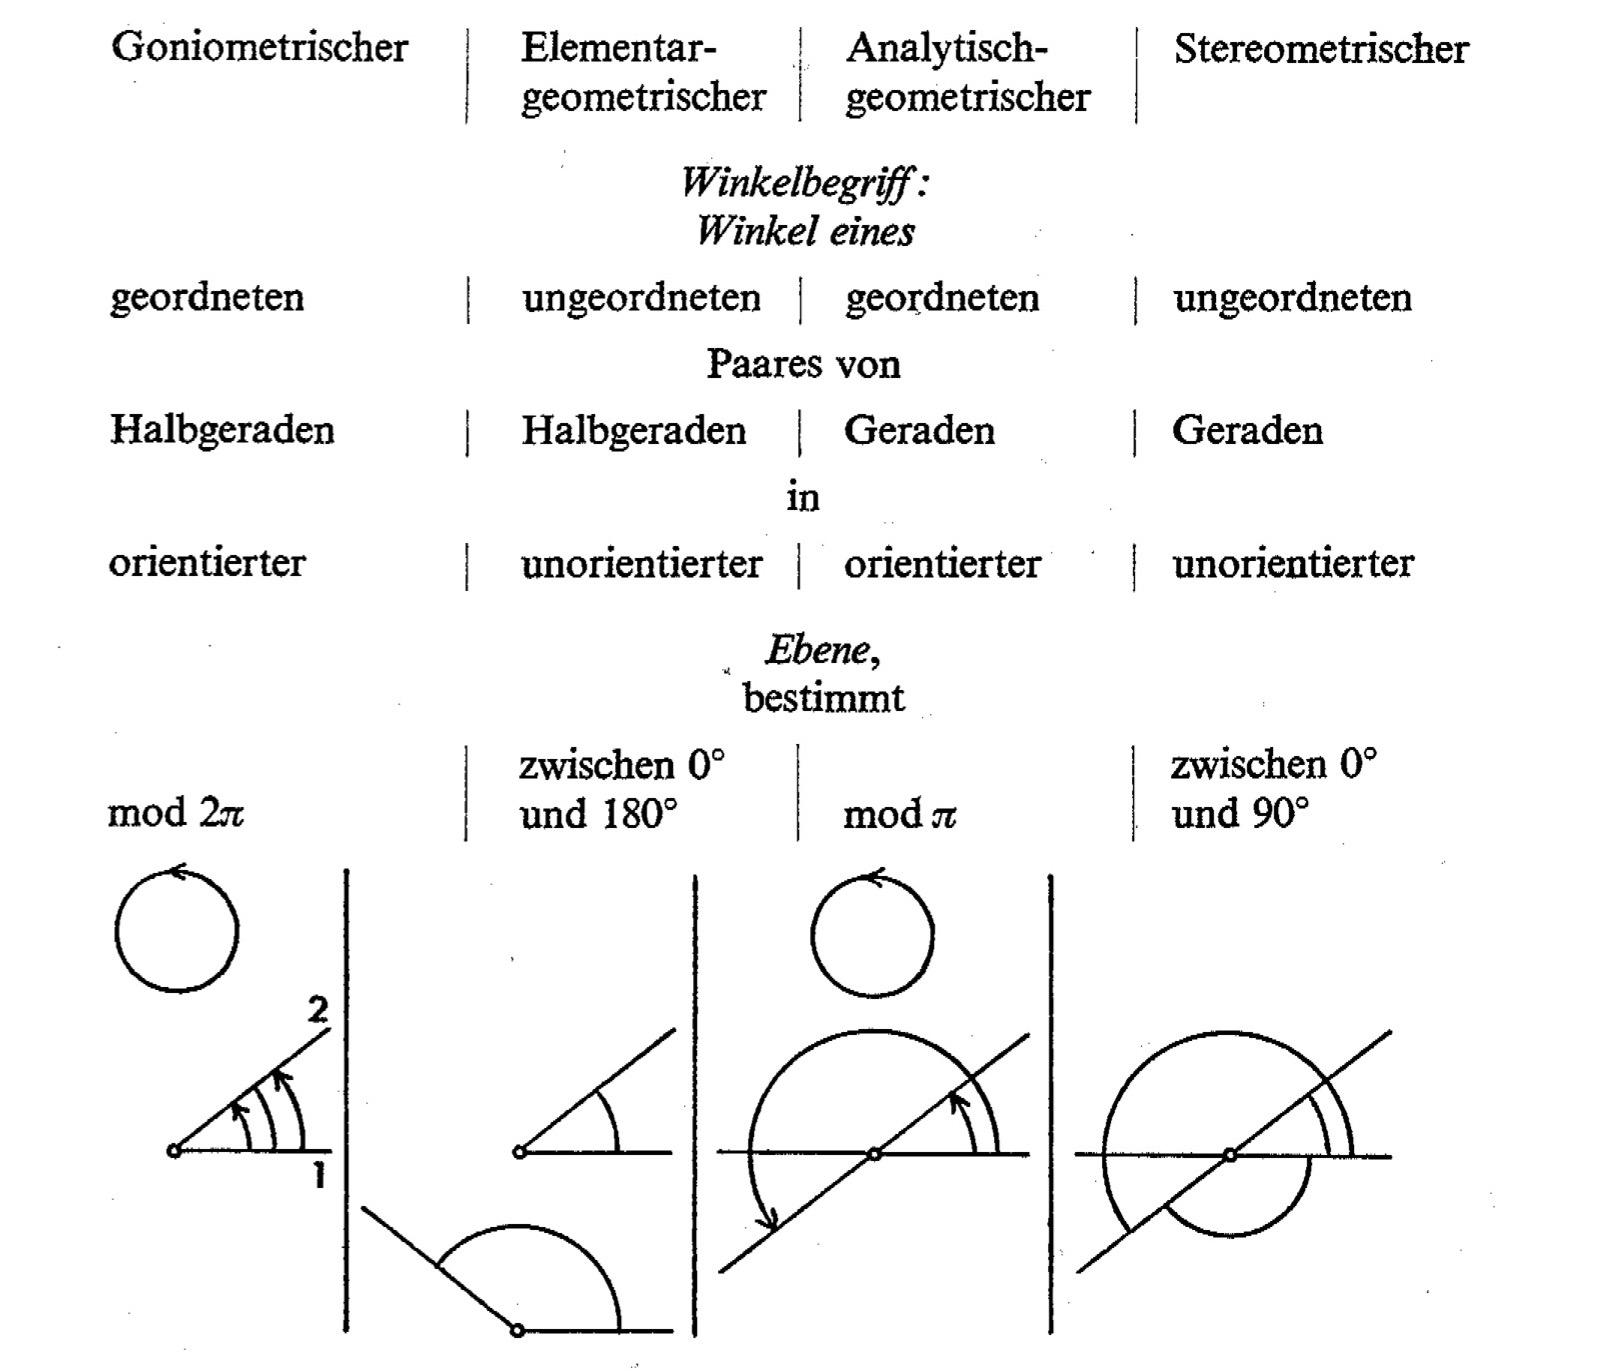
\includegraphics[width=0.75\linewidth]{pictures/1-FreudenthalWinkel} 

}

\caption{Winkelbegriffe nach Freudenthal (\protect\hyperlink{ref-Freudenthal:1973}{1973, S. 441})}\label{fig:FreudenthalWinkel}
\end{figure}

Er diskutiert, welchen Einfluss die jeweilige Sichtweise auf dem Maßbereich hat, wie Winkel überhaupt gemessen werden können und wie mit Winkeln operiert werden kann. Was passiert denn, wenn man ein geordnetes Strahlenpaar in der orientierten Ebene spiegelt (vgl. \protect\hyperlink{ref-Freudenthal:1973}{Freudenthal, 1973, S. 443~ff.})?

Wenn die Reihenfolge der Strahlen erhalten bleibt und die Winkelmessung aufgrund der Orientierung der Ebene vorgegeben ist, ändert sich damit ggf. auch das Maß des Winkels (siehe Abbildung \ref{fig:FreudenthalWinkelSpiegeln}).



\begin{figure}

{\centering 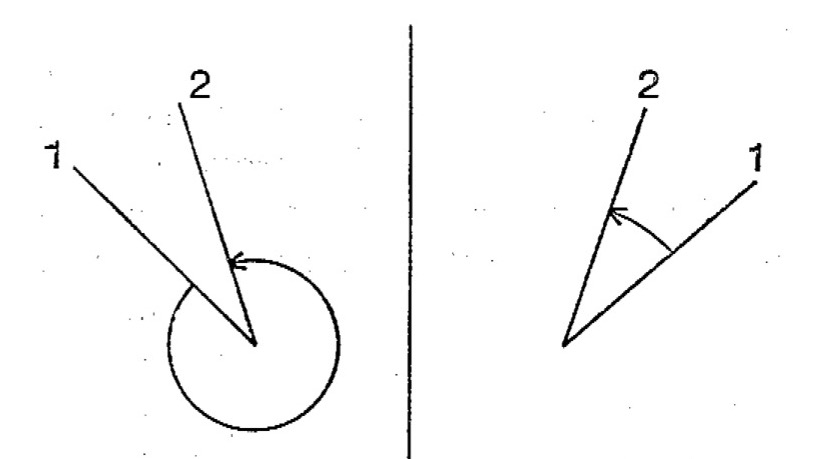
\includegraphics[width=0.5\linewidth]{pictures/1-FreudenthalWinkelSpiegeln} 

}

\caption{Spiegelung eines goniometrischen Winkels (\protect\hyperlink{ref-Freudenthal:1973}{Freudenthal, 1973, S. 443})}\label{fig:FreudenthalWinkelSpiegeln}
\end{figure}

Hierzu stellt Freudenthal (\protect\hyperlink{ref-Freudenthal:1973}{1973, S. 443~ff.}) weitere fachmathematische Ausführungen dar und schließt damit, dass der elementargeometrische, goniometrische und analytische Winkelbegriff aus fachlicher Sicht für den schulischen Lernpfad unentbehrlich sind (\protect\hyperlink{ref-Freudenthal:1973}{Freudenthal, 1973, S. 449}).

Die \emph{Spezifizierung} besteht also darin, den Begriff zu schärfen und Operationen mit ihm zu beschreiben. Die \emph{Strukturierung} besteht u.~a. in der vernetzenden Analyse der verschiedenen Winkelbegriffe und der Schlussfolgerung ihrer gleichermaßen Bedeutsamkeit für den Schulunterricht.

\hypertarget{semantische-ebene}{%
\subsection{Semantische Ebene}\label{semantische-ebene}}

Dazu, welche Vorstellungen Schülerinnen und Schüler zum Winkelbegriff entwickeln sollen, sei u.~a. auf Krainer (\protect\hyperlink{ref-Krainer:1989}{1989}) und Mitchelmore \& White (\protect\hyperlink{ref-Mitchelmore:1998}{1998}) verwiesen. Eine grundsätzliche Schwierigkeit beim Unterrichten von Winkeln sind diverse und (scheinbar) nicht in Verbindung zu bringende Anwendungskontexte, die dennoch über denselben mathematischen Begriff beschrieben werden können. So ist das Sichtfeld eines Tieres ebenso wie die Umdrehung eines Wasserzählers über Winkel beschreibbar -- haben doch beide Situationen zunächst nichts miteinander zu tun.

Aufbauend auf den Arbeiten von Krainer (\protect\hyperlink{ref-Krainer:1989}{1989}) und Mitchelmore \& White (\protect\hyperlink{ref-Mitchelmore:1998}{1998}) können über eine Verknüpfung zur formalen Ebene mithilfe einer \emph{informationstheoretischen Winkeldefinition} (\protect\hyperlink{ref-Etzold2021}{Etzold, 2021, S. 39~f..}) vier Grundvorstellungen zum Winkelbegriff ausgearbeitet bzw. validiert werden:

\begin{itemize}
\tightlist
\item
  Winkel als Knick
\item
  Winkel als Feld
\item
  Winkel als Richtungsänderung
\item
  Winkel als Umdrehung
\end{itemize}

Dabei erhalten die \emph{Bestandteile} eines Winkels (Scheitelpunkt, Schenkel, ggf. Bereich zwischen den Schenkeln, Abweichungsmaß) eine besondere Bedeutung, über die sich auch eine sinnvolle Reihenfolge der Behandlung dieser Grundvorstellungen ableiten lässt. So »bietet es sich an, mit den Winkelfeldern zu beginnen. Bei diesen werden die meisten Bestandteile sichtbar (Scheitelpunkt, beide Schenkel als Begrenzungen sowie der zwischen den Schenkeln relevante Bereich) {[}\ldots{]}. Anschließend können Knicke oder Richtungsänderungen behandelt werden, woraufhin die Umdrehungen folgen.« (\protect\hyperlink{ref-Etzold2021}{Etzold, 2021, S. 60})

Die \emph{Spezifizierung} in diesem semantischen Teil ist demnach die Ausarbeitung der Grundvorstellungen. Die Begründung einer möglichen Reihenfolge kann der \emph{Strukturierung} des Lerngegenstands zugeordnet werden.

\hypertarget{konkrete-ebene}{%
\subsection{Konkrete Ebene}\label{konkrete-ebene}}

Um die einzelnen Vorstellungen zu Winkeln aufzubauen, bedarf es charakteristischer Situationen, an denen der mathematische Kern der jeweiligen Vorstellung besonders gut sichtbar wird. Abbildung \ref{fig:Winkelsituationen} zeigt derartige \emph{Winkelsituationen} und die zugehörigen Grundvorstellungen (hier \emph{Winkelkontexte}).



\begin{figure}

{\centering 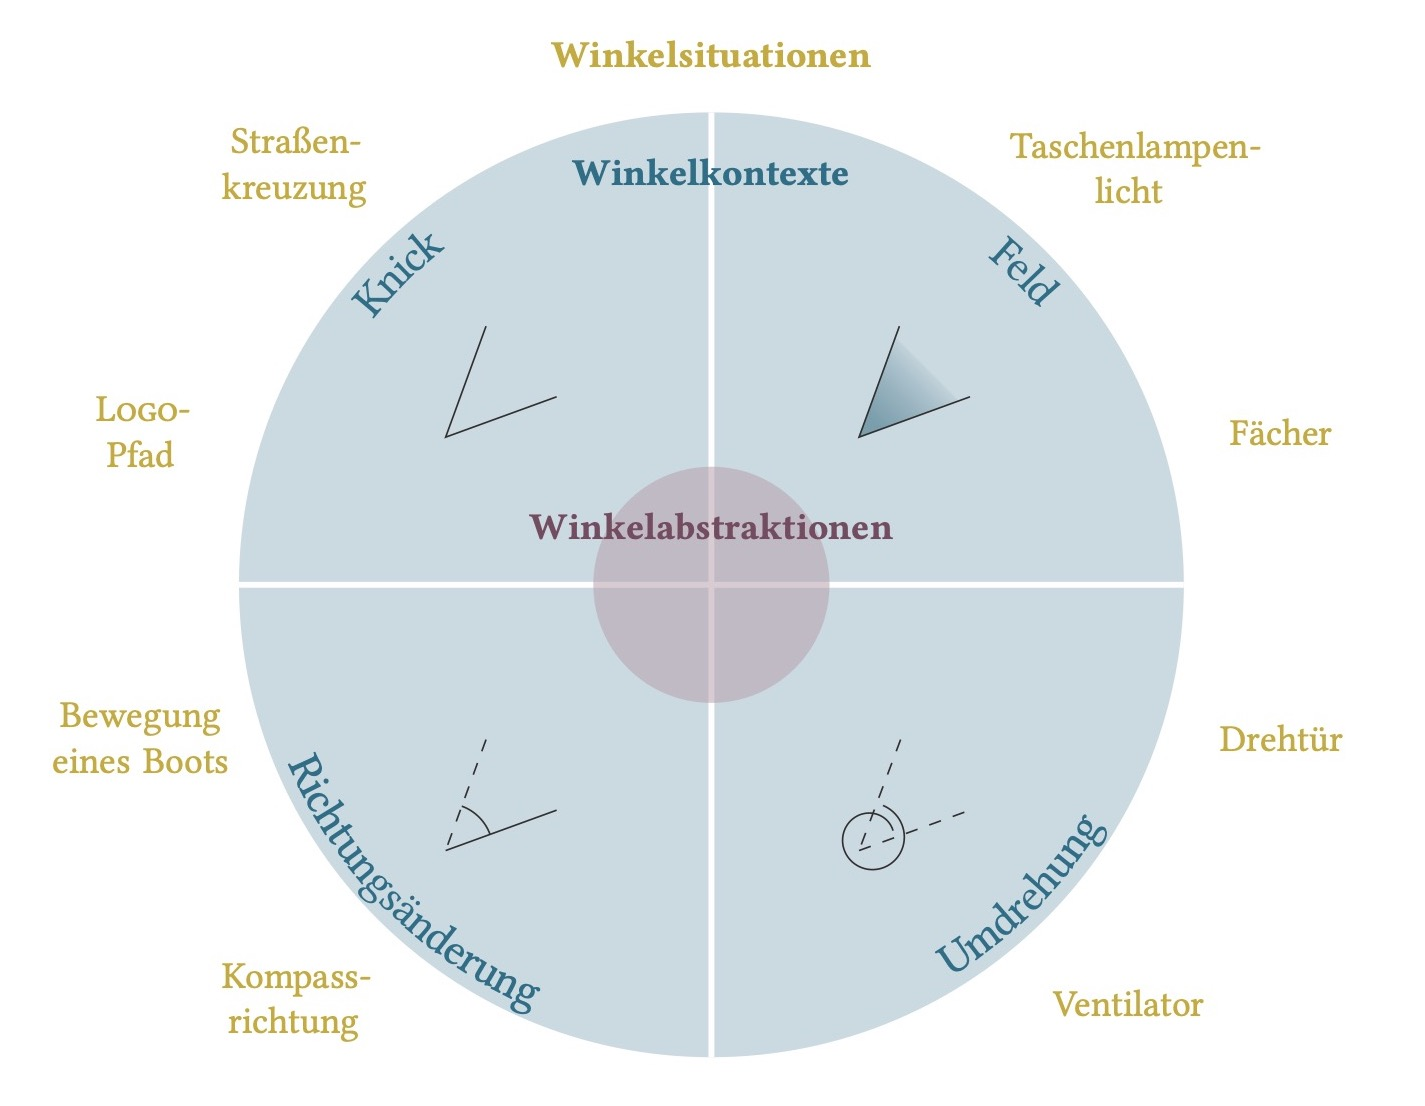
\includegraphics[width=0.75\linewidth]{pictures/1-Winkelsituationen} 

}

\caption{Winkelsituationen und -kontexte (\protect\hyperlink{ref-Etzold2021}{Etzold, 2021, S. 70})}\label{fig:Winkelsituationen}
\end{figure}

Exemplarisch für die Grundvorstellung des Winkels als Feld wird darauf aufbauend eine Lernumgebung und darin eingebettetes Unterrichtsmaterial entwickelt, mithilfe dessen die Grundvorstellung ausgebildet werden kann. An der konkreten Situation der \emph{Sichtfelder von Tieren} sollen die Schülerinnen und Schüler Handlungen ausführen, die es ihnen ermöglicht, den mathematischen Kern hinter dem konkreten Beispiel zu erkunden.

Die Schülerinnen und Schüler nutzen dazu eine App (siehe Abbildung \ref{fig:WinkelfarmApp}), in der mehrere Tiere mit ihren Sichtfeldern dargestellt werden können, und erhalten u.~a. folgende Aufgaben (vgl. \protect\hyperlink{ref-Etzold:2019Praxis4}{Etzold, 2019b, S. 8~ff.}):

\begin{enumerate}
\def\labelenumi{\arabic{enumi}.}
\tightlist
\item
  Setze das Schaf an eine Stelle, an der es von der Kuh gesehen wird, aber die Kuh selbst nicht sieht.
\item
  Setze das Schaf an eine Stelle, an der es nicht von der Kuh gesehen wird.
\item
  Das Schaf will die Kuh verwirren. Bewege es an möglichst viele Orte, an denen es von der Kuh gesehen wird.
\item
  Setze das Schaf an eine Stelle, an der es noch gerade so von der Kuh gesehen wird.
\item
  Wo muss das Schaf lang laufen, damit es die gesamte Zeit gerade so von der Kuh gesehen wird?
\end{enumerate}

An Aufgabe 5 kann z.~B. erkundet werde, dass sich das Schaf geradlinig auf der Grenze zwischen Sichtfeld und Nicht-Sichtfeld bewegen muss. In die eine Richtung ist die Bewegung beliebig fortsetzbar, in die andere durch den Kopf der Kuh begrenzt. Eine mathematische Verallgemeinerung dieser Handlung besteht dann in der Identifizierung des Schenkels (Begrenzung) als Strahl (nur in eine Richtung fortsetzbar) mit dem Scheitelpunkt (Kopf der Kuh) als \emph{Quelle} des Winkelfeldes.



\begin{figure}

{\centering 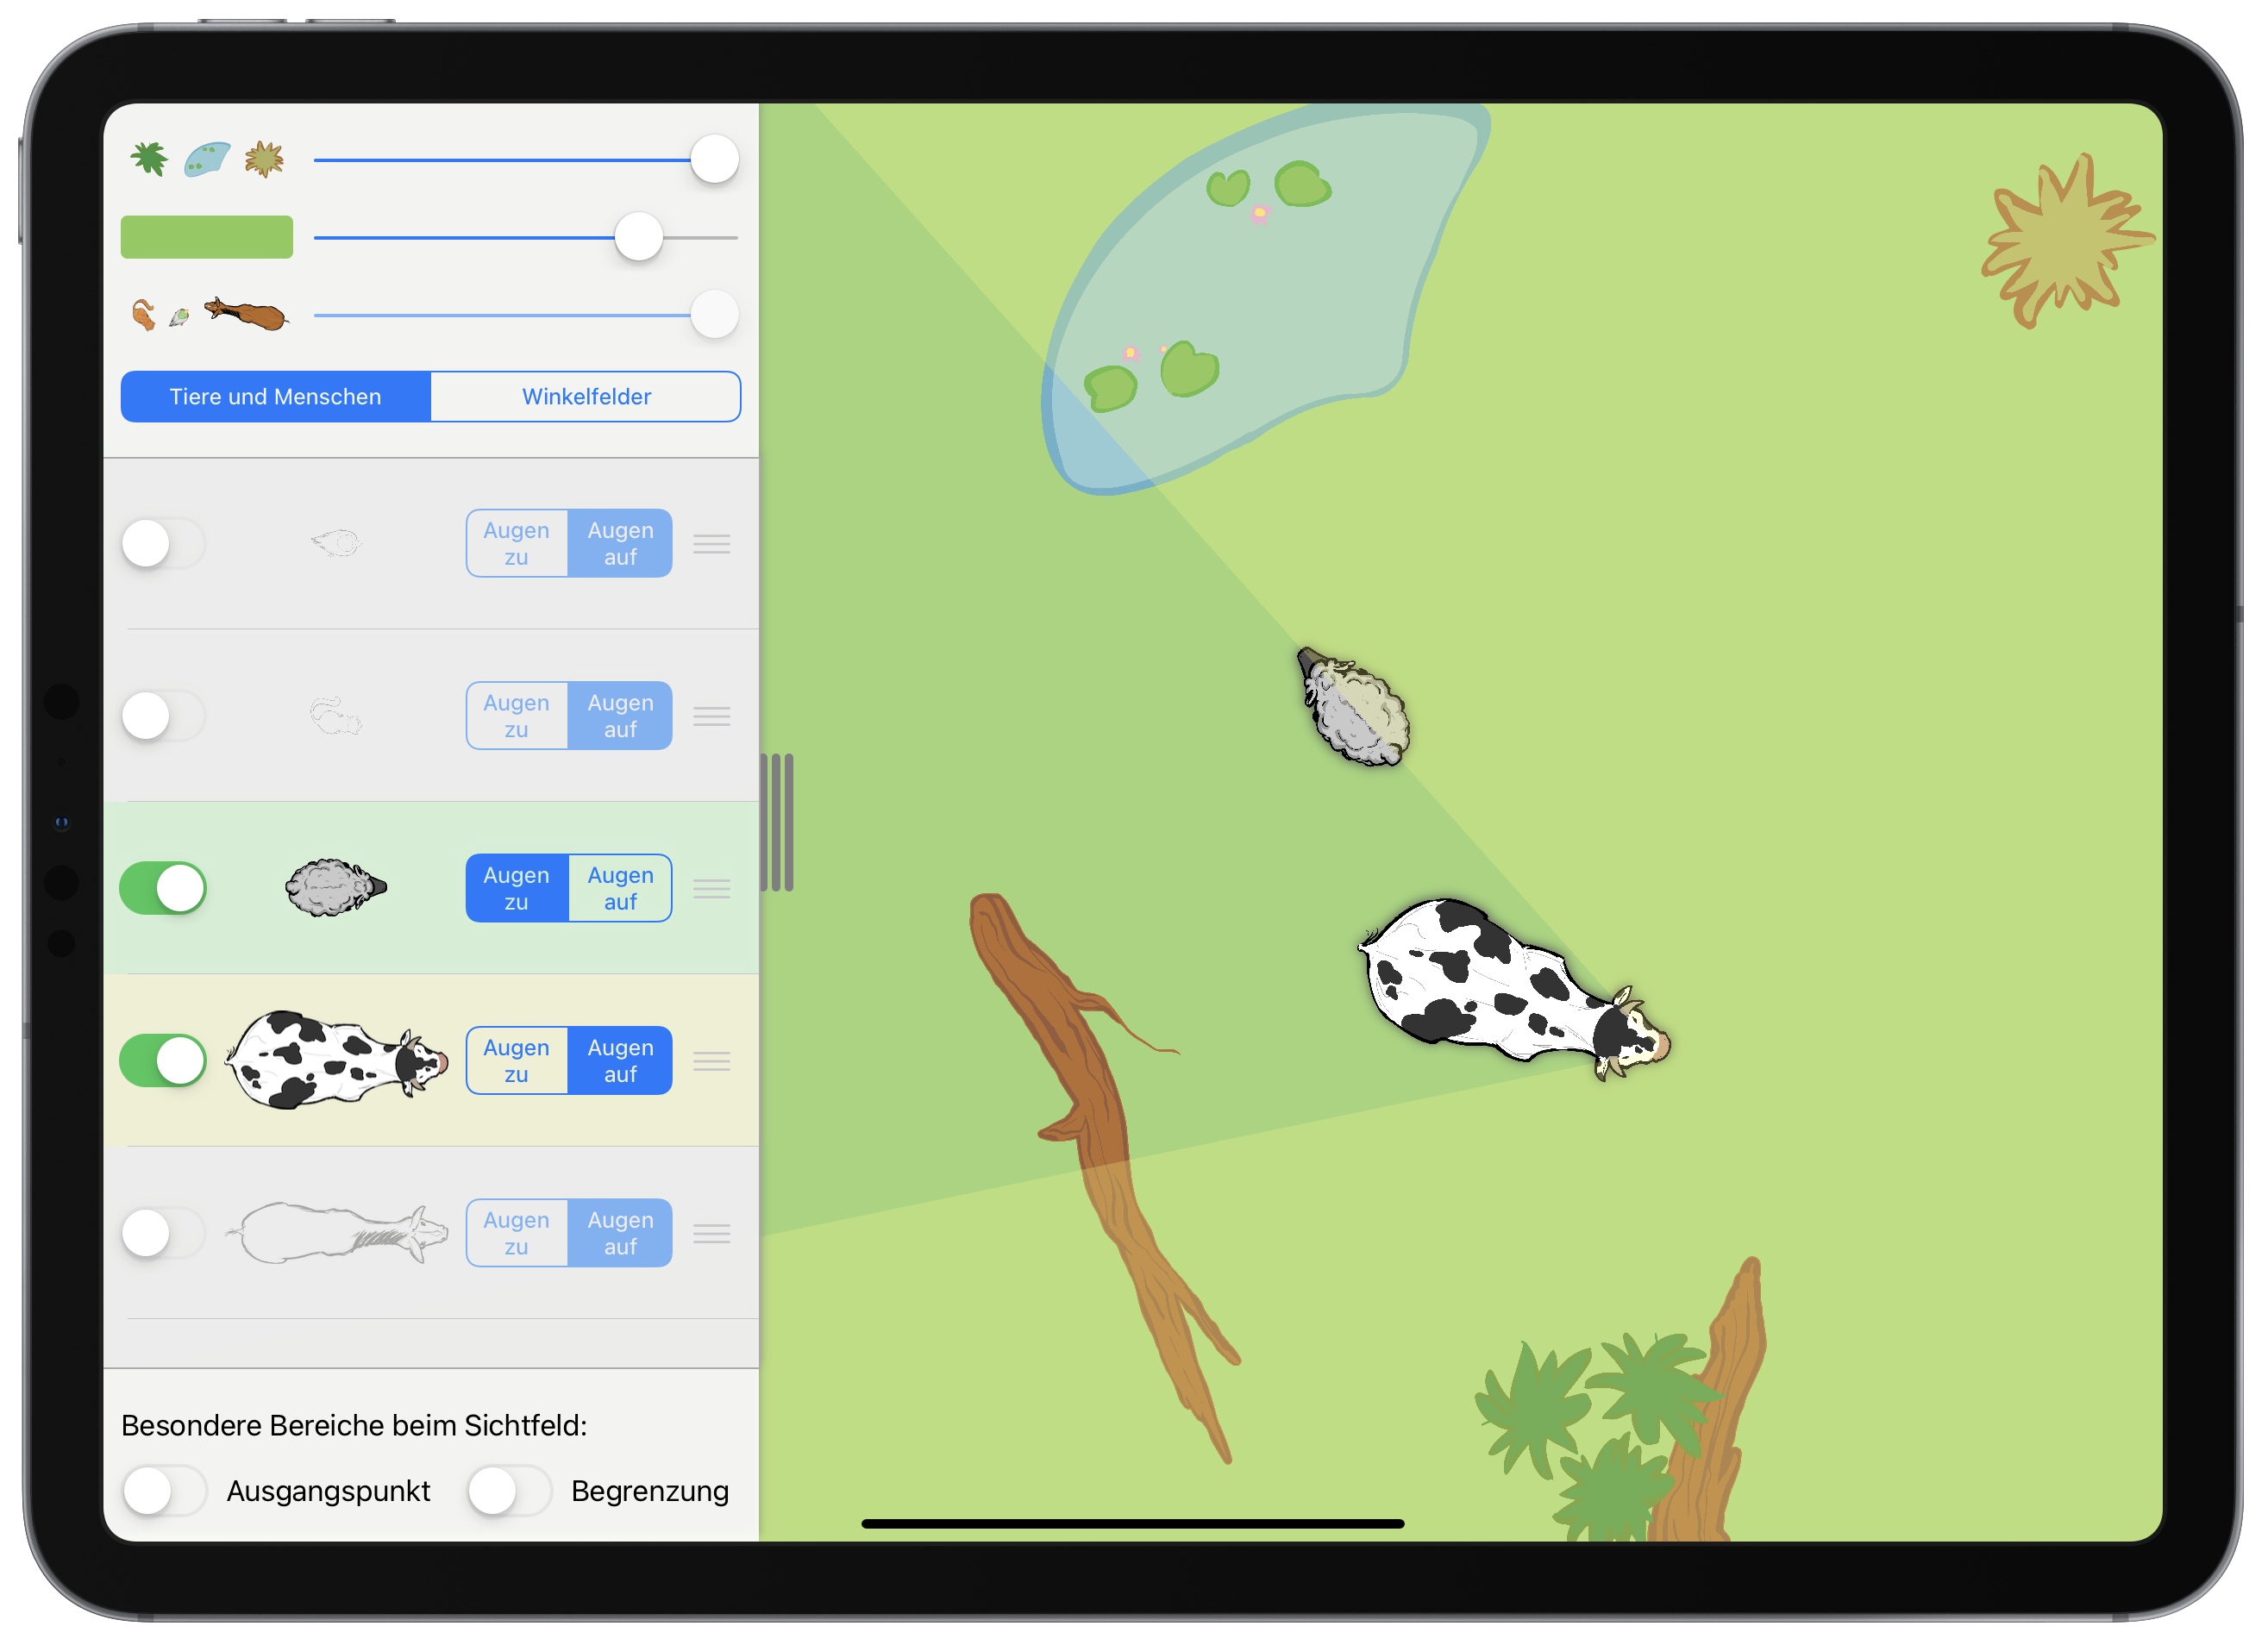
\includegraphics[width=0.75\linewidth]{pictures/1-Winkelfarm} 

}

\caption{Screenshot der App Winkel-Farm (\protect\hyperlink{ref-Etzold:2019}{Etzold, 2019a})}\label{fig:WinkelfarmApp}
\end{figure}

Als \emph{Spezifizierung} kann das Finden der Sichtfeld-Situation als charakterisches Beispiel für ein Winkelfeld angesehen werden. Die \emph{Strukturierung} führt zum dargestellten Lernpfad und den konkreten Aufgabenstellung, über die konkrete Handlungen verallgemeinert werden und damit das mathematische Verständnis aufgebaut wird.

\hypertarget{empirische-ebene}{%
\subsection{Empirische Ebene}\label{empirische-ebene}}

Die zuvor beschriebene Lernumgebung wurde in mehreren Zyklen erprobt und dabei die Qualität der Handlungen der Schülerinnen und Schüler beobachtet. Ein Ziel bestand darin, dass möglichst verallgemeinerbare Handlungen (wie oben am Beispiel des Schenkels beschrieben) durchgeführt werden.

Es wird erwartet, dass die Repräsentation eines Sichtfeldes von der Draufsicht über eine semintransparent ausgemalte Teilfläche der Ebene noch nicht bekannt ist. Um diese nachzuvollziehen und mit eigenen Erfahrungen in Bezug zu bringen, wird an den Beginn der Unterrichtsstunde ein Bild des Klassenraumes in der Draufsicht präsentiert (siehe Abbildung \ref{fig:Klassenraum}). Dann soll eine Schülerin oder ein Schüler beschreiben, was sie/er alles sieht, ohne den Kopf zu drehen. Dieser Bereich wird auf dem Bild eingezeichnet, so dass die Repräsentation des Sichtfeldes im Folgenden zur Verfügung steht.

\begin{figure}

{\centering 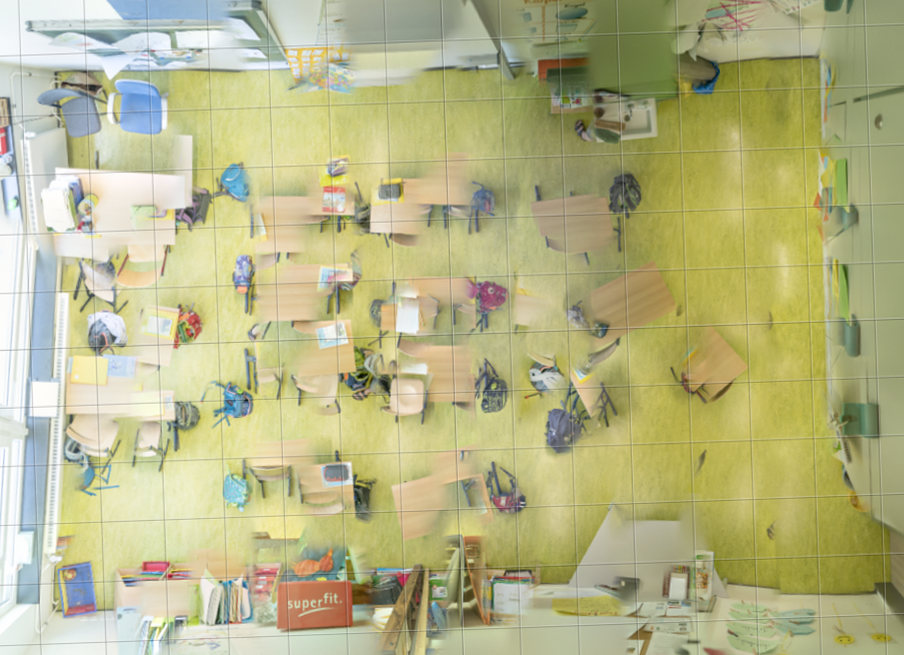
\includegraphics[width=0.75\linewidth]{pictures/1-Klassenraum} 

}

\caption{Klassenraum von oben (Foto: Christian Dohrmann)}\label{fig:Klassenraum}
\end{figure}

In der Erprobung konnte beobachtet werden, dass einige Bedienschwierigkeiten mit der Anwendung den Lernfortschritt hemmten. Dies konnte u.~a. dadurch verbessert werden, dass vor die eigentliche Erarbeitung eine freie Erkundungsphase mit der App (siehe Abbildung \ref{fig:WinkelfarmStart}) gesetzt wurde (\protect\hyperlink{ref-Etzold2021}{Etzold, 2021, S. 147, 152}). Durch spezifische Aufgabenstellungen wurden bestimmte Funktionen der App fokussiert:

\begin{figure}

{\centering 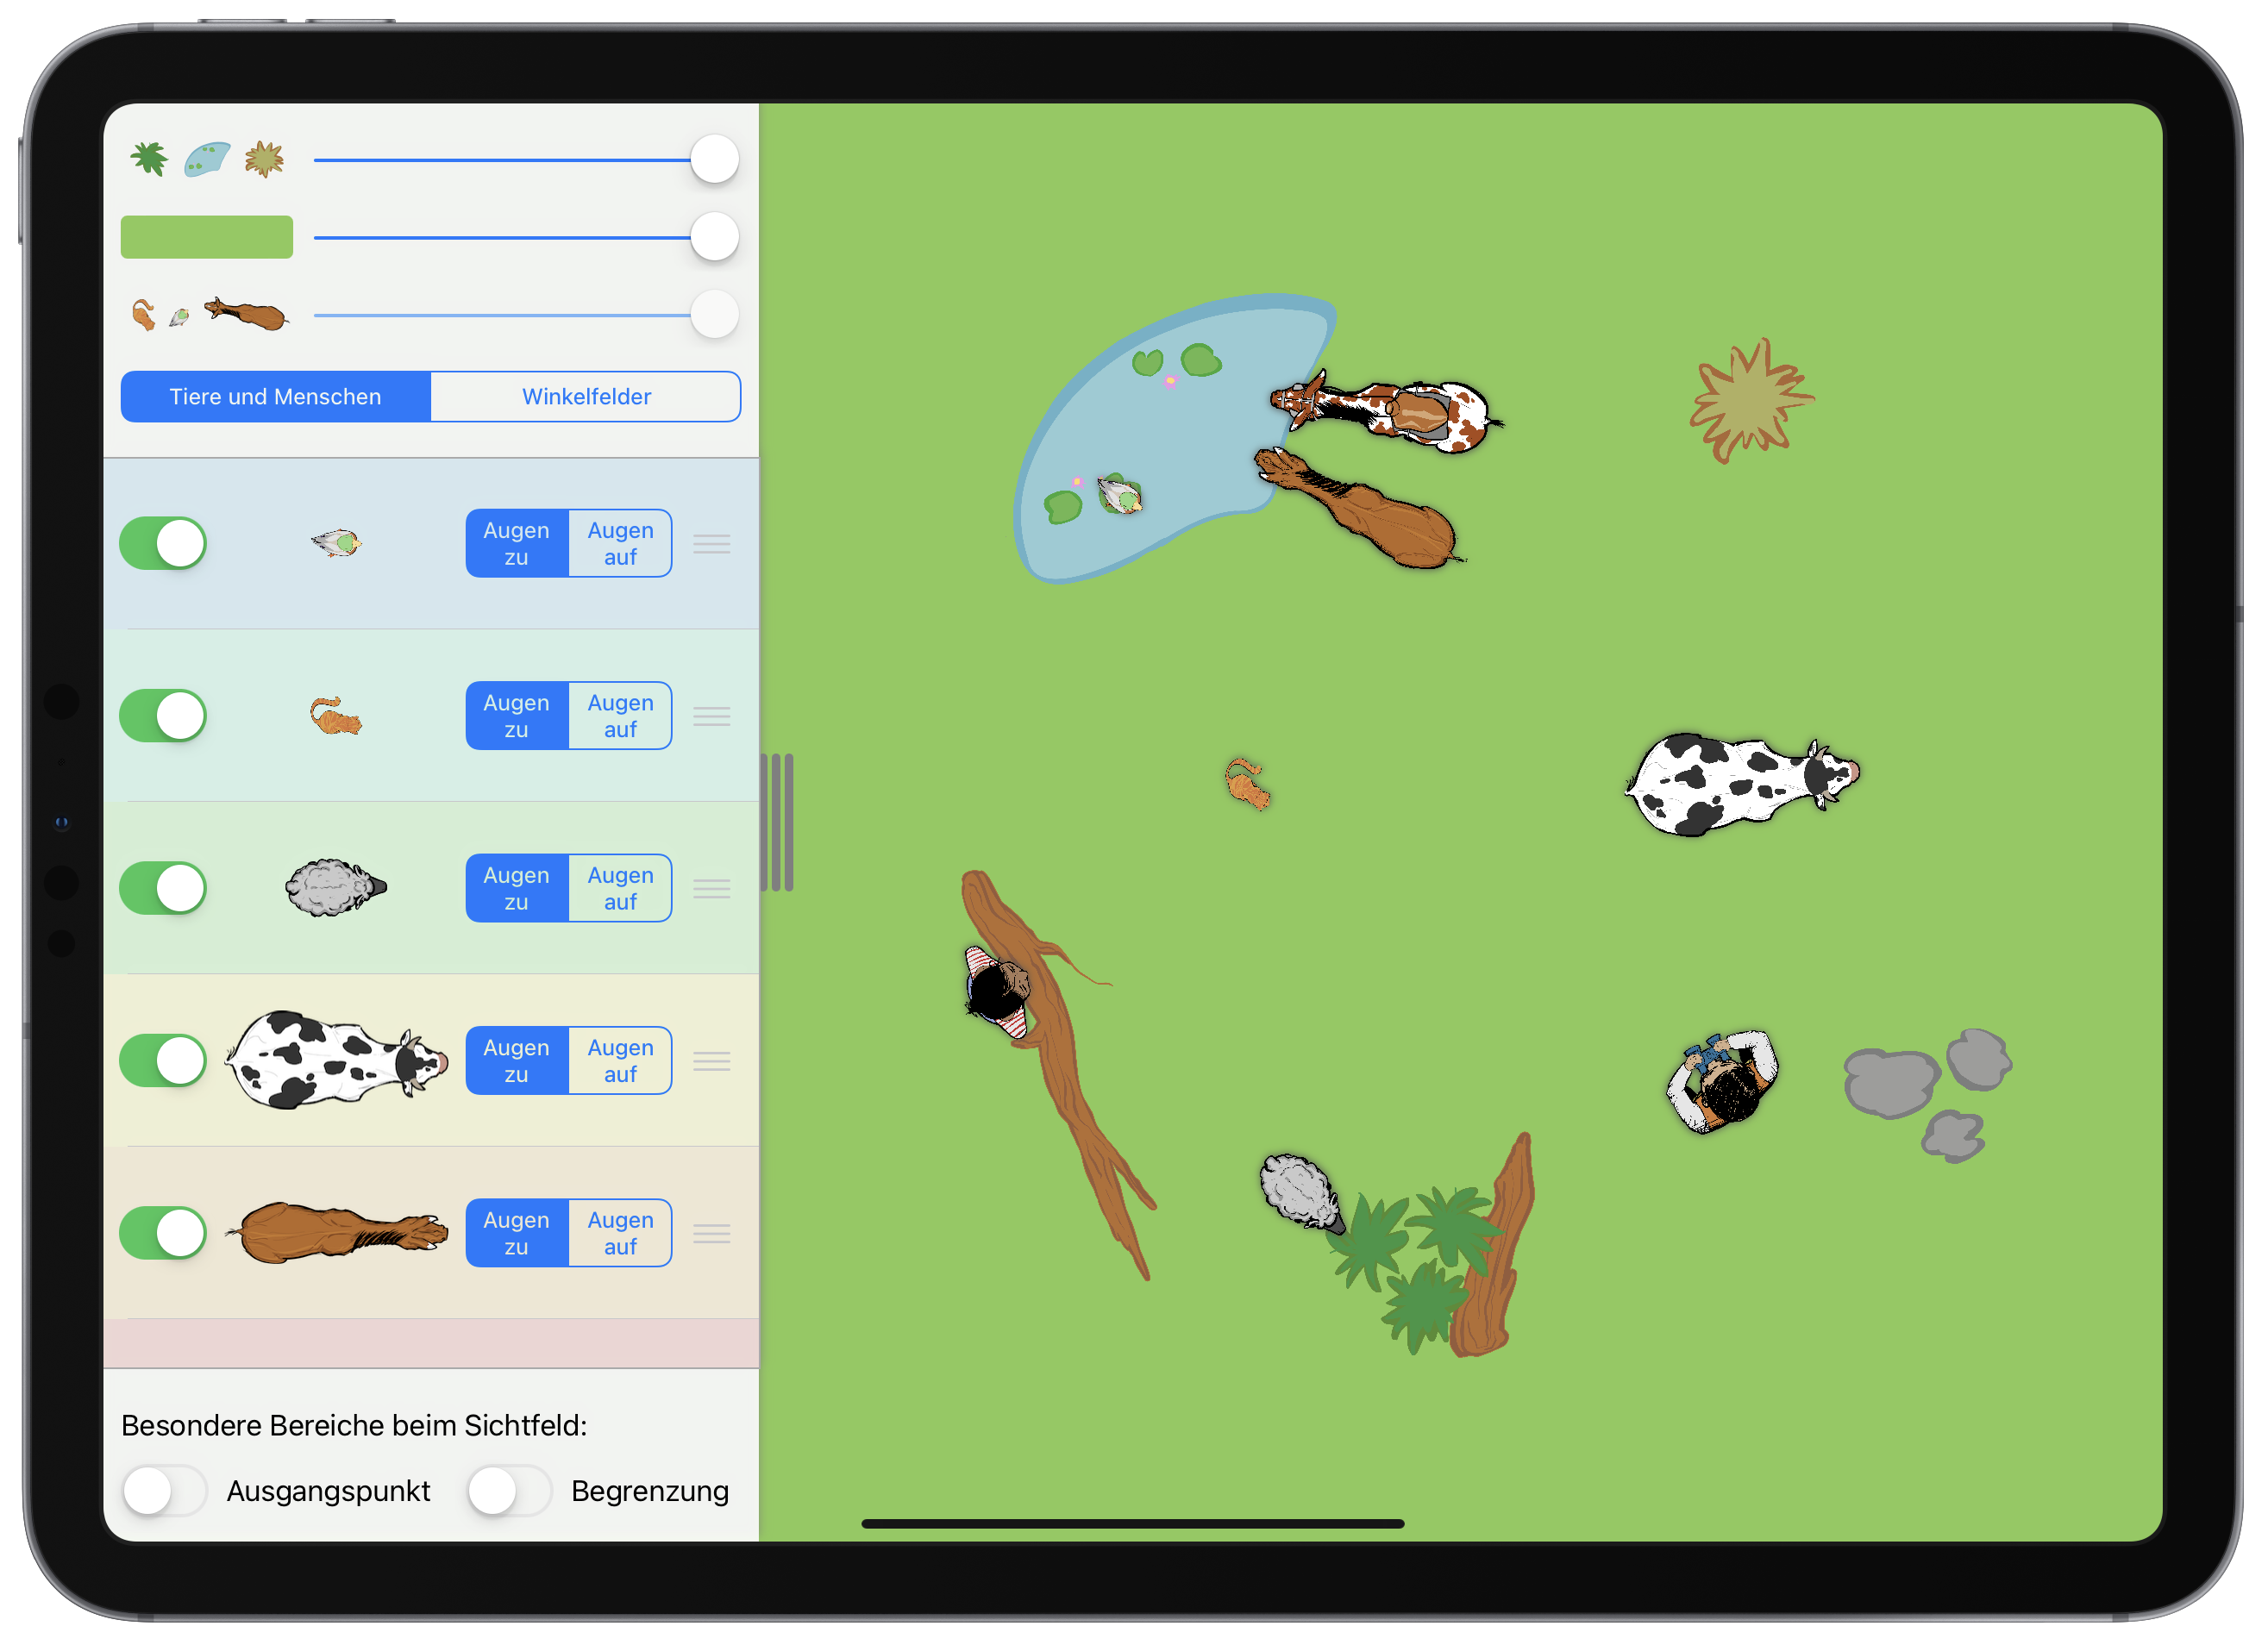
\includegraphics[width=0.75\linewidth]{pictures/1-WinkelfarmStart} 

}

\caption{Möglicher Startbildschirm für die freie Erkundungphase}\label{fig:WinkelfarmStart}
\end{figure}

\emph{»Das Pferd soll auf dem Steinpflaster stehen, die Frau soll auf dem Pferd sitzen/stehen. Das Pferd guckt in Richtung der grünen Büsche, die Frau hat die Augen zu. Gleichzeitig versteckt sich die Katze unter der Kuh.«}

Die Einführungsphase über das Klassenraumfoto folgt aus der \emph{Spezifizierung} innerhalb der empirischen Ebene. Das Hinzufügen der freien Erkundungsphase ist dagegen der \emph{Strukturierung} der Analyse zuzuordnen.

\hypertarget{verknuxfcpfung-der-ebenen}{%
\subsection{Verknüpfung der Ebenen}\label{verknuxfcpfung-der-ebenen}}

An den Ausführungen ist schon sichtbar geworden, dass sich die Ebenen nicht immer trennen lassen und teilweise gegenseitig beeinflussen. Auch gehen oft Spezifizierung und Strukturierung ineinander über.

Das ist aber gar nicht schlimm, ganz im Gegenteil. Es zeigt wieder einmal, wie wichtig solch ein ganzheitlicher Ansatz ist, so dass eine stoffdidaktische Analyse aus den diversen Sichtpunkten heraus betrachtet werden sollte.

Wichtig ist v.~a., dass Sie sich als Lehrkraft stets darüber im Klaren sind, dass für eine stoffdidaktische Analyse verschiedene Perspektiven verfolgt werden müssen. Sehen Sie den Vier-Ebenen-Ansatz daher auch als Kontrollinstrument, ob Sie an alles gedacht haben, wenn Sie einen Lerngegenstand intensiv analysieren.

\hypertarget{vier-ebenen-nachbereitung}{%
\section{Zum Nachbereiten}\label{vier-ebenen-nachbereitung}}

\begin{enumerate}
\def\labelenumi{\arabic{enumi}.}
\tightlist
\item
  Lesen Sie den Artikel von Hußmann \& Prediger (\protect\hyperlink{ref-Hussmann:2016}{2016}) zum Vier-Ebenen-Ansatz.
\item
  Reflektieren Sie Ihre bisherige Fach- und Fachdidaktikausbildung in Mathematik dahingehend, welche der aufgeworfenen Fragen Sie zu konkreten Themenbereichen (nicht) beantworten könnten.
\end{enumerate}

\hypertarget{fundamentale-ideen}{%
\chapter{Fundamentale Ideen}\label{fundamentale-ideen}}

\hypertarget{grundvorstellungen}{%
\chapter{Grundvorstellungen}\label{grundvorstellungen}}

\hypertarget{kernideen-kernfragen-kontexte}{%
\chapter{Kernideen, Kernfragen, Kontexte}\label{kernideen-kernfragen-kontexte}}

\hypertarget{erstes-intermezzo}{%
\chapter{\texorpdfstring{Erstes Intermezzo }{Erstes Intermezzo }}\label{erstes-intermezzo}}

\hypertarget{part-lernprozesse-gestalten}{%
\part*{Lernprozesse gestalten}\label{part-lernprozesse-gestalten}}
\addcontentsline{toc}{part}{Lernprozesse gestalten}

\hypertarget{lernhandlungen}{%
\chapter{Lernhandlungen}\label{lernhandlungen}}

\hypertarget{arbeitsmittel}{%
\chapter{Arbeitsmittel}\label{arbeitsmittel}}

\hypertarget{aufgabengestaltung}{%
\chapter{Aufgabengestaltung}\label{aufgabengestaltung}}

\hypertarget{zweites-intermezzo}{%
\chapter{\texorpdfstring{Zweites Intermezzo }{Zweites Intermezzo }}\label{zweites-intermezzo}}

\hypertarget{part-inhaltsbezogene-kompetenzen}{%
\part*{Inhaltsbezogene Kompetenzen}\label{part-inhaltsbezogene-kompetenzen}}
\addcontentsline{toc}{part}{Inhaltsbezogene Kompetenzen}

\hypertarget{leitidee-zahl-und-operation}{%
\chapter{Leitidee Zahl und Operation}\label{leitidee-zahl-und-operation}}

\hypertarget{leitidee-messen-und-gruxf6uxdfen}{%
\chapter{Leitidee Messen und Größen}\label{leitidee-messen-und-gruxf6uxdfen}}

\hypertarget{leitidee-raum-und-form}{%
\chapter{Leitidee Raum und Form}\label{leitidee-raum-und-form}}

\hypertarget{leitidee-strukturen-und-funktionaler-zusammenhang}{%
\chapter{Leitidee Strukturen und funktionaler Zusammenhang}\label{leitidee-strukturen-und-funktionaler-zusammenhang}}

\hypertarget{leitidee-daten-und-zufall}{%
\chapter{Leitidee Daten und Zufall}\label{leitidee-daten-und-zufall}}

\hypertarget{appendix-anhang}{%
\appendix}


\hypertarget{seminar-und-hausarbeit}{%
\chapter{Seminar und Hausarbeit}\label{seminar-und-hausarbeit}}

\hypertarget{vollstuxe4ndiges-literaturverzeichnis}{%
\chapter{Vollständiges Literaturverzeichnis}\label{vollstuxe4ndiges-literaturverzeichnis}}

\hypertarget{refs}{}
\begin{CSLReferences}{1}{0}
\leavevmode\vadjust pre{\hypertarget{ref-Etzold:2019}{}}%
Etzold, H. (2019a). \emph{Winkel-{Farm}} (Version 2) {[}App{]}. \url{https://apps.apple.com/de/app/winkel-farm/id1369585218}

\leavevmode\vadjust pre{\hypertarget{ref-Etzold:2019Praxis4}{}}%
Etzold, H. (2019b). \emph{Winkel-{Farm} -- {Leitfaden} für {Lehrerinnen} und {Lehrer}} (Version 2). Zenodo. \url{https://doi.org/10.5281/zenodo.4747700}

\leavevmode\vadjust pre{\hypertarget{ref-Etzold2021}{}}%
Etzold, H. (2021). \emph{Neue Zugänge zum Winkelbegriff} {[}Dissertation, Universität Potsdam{]}. \url{https://doi.org/10.25932/publishup-50418}

\leavevmode\vadjust pre{\hypertarget{ref-Freudenthal:1973}{}}%
Freudenthal, H. (1973). \emph{Mathematik als pädagogische {Aufgabe}} (Bd. 2). Klett.

\leavevmode\vadjust pre{\hypertarget{ref-Hefendehl-Hebeker:2016}{}}%
Hefendehl-Hebeker, L. (2016). Subject-matter didactics in {German} traditions: {Early} historical developments. \emph{Journal für Mathematik-Didaktik}, \emph{37}(S1), 11--31. \url{https://doi.org/10.1007/s13138-016-0103-7}

\leavevmode\vadjust pre{\hypertarget{ref-Hussmann:2016}{}}%
Hußmann, S., \& Prediger, S. (2016). Specifying and Structuring Mathematical Topics: A Four-Level Approach for Combining Formal, Semantic, Concrete, and Empirical Levels Exemplified for Exponential Growth. \emph{Journal für Mathematik-Didaktik}, \emph{37}(S1), 33--67. \url{https://doi.org/10.1007/s13138-016-0102-8}

\leavevmode\vadjust pre{\hypertarget{ref-Hussmann:2016a}{}}%
Hußmann, S., Rezat, S., \& Sträßer, R. (2016). Subject {Matter} {Didactics} in {Mathematics} {Education}. \emph{Journal für Mathematik-Didaktik}, \emph{37}(S1), 1--9. \url{https://doi.org/10.1007/s13138-016-0105-5}

\leavevmode\vadjust pre{\hypertarget{ref-Jahnke:2010}{}}%
Jahnke, T. (2010). Vom mählichen {Verschwinden} des {Fachs} aus der {Mathematikdidaktik}. \emph{GDM-Mitteilungen 89}, 21--24. \url{https://ojs.didaktik-der-mathematik.de/index.php/mgdm/article/view/559/550}

\leavevmode\vadjust pre{\hypertarget{ref-Krainer:1989}{}}%
Krainer, K. (1989). \emph{Lebendige {Geometrie}. Überlegungen zu einem integrativen {Verständnis} von {Geometrieunterricht} anhand des {Winkelbegriffs}} {[}Dissertation{]}. Alpen-Adria-Universität Klagenfurt.

\leavevmode\vadjust pre{\hypertarget{ref-Mitchelmore:1990}{}}%
Mitchelmore, M. (1990). Psychologische und mathematische Schwierigkeiten beim Lernen des Winkelbegriffs. \emph{mathematica didactica}, \emph{13}, 19--37.

\leavevmode\vadjust pre{\hypertarget{ref-Mitchelmore:1998}{}}%
Mitchelmore, M., \& White, P. (1998). Development of {Angle} {Concepts}: {A} {Framework} for {Research}. \emph{Mathematics Education Research Journal}, \emph{10}(3), 4--27.

\leavevmode\vadjust pre{\hypertarget{ref-Schupp:2016}{}}%
Schupp, H. (2016). Gedanken zum „{Stoff}`` und zur „{Stoffdidaktik}`` sowie zu ihrer {Bedeutung} für die {Qualität} des {Mathematikunterrichts}. \emph{Mathematische Semesterberichte}, \emph{63}(1), 69--92. \url{https://doi.org/10.1007/s00591-016-0159-y}

\leavevmode\vadjust pre{\hypertarget{ref-Strehl:1983}{}}%
Strehl, R. (1983). Anschauliche {Vorstellung} und mathematische {Theorie} beim {Winkelbegriff}. \emph{mathematica didactica}, \emph{6}, 129--146.

\leavevmode\vadjust pre{\hypertarget{ref-Wittmann:2015}{}}%
Wittmann, E. C. (2015). Strukturgenetische didaktische {Analysen} -- empirische {Forschung} „erster {Art}``. \emph{mathematica didactica}, 239--255. \url{http://www.mathematica-didactica.com/altejahrgaenge/md_2015/md_2015_Wittmann_Stoffdidaktik.pdf}

\end{CSLReferences}

\end{document}
